
\usepackage{tikz}
\usepackage[utf8]{inputenc}
\usepackage{amsmath}
\usepackage{amsfonts}
\usepackage{amssymb}
\usepackage{stackrel}
%\usepackage{kpfonts}
\usepackage{amssymb, amsmath, amsbsy} 
\usepackage{makeidx}
\usepackage{graphicx}
\usepackage{multicol}
\usepackage{changepage}
\usepackage{float}
\usepackage{cite}
\usepackage{lipsum}
\usepackage{pstricks, caption}
\usepackage{url}
\usepackage[spanish, es-tabla]{babel}
\usepackage[shortlabels]{enumitem}
\usepackage{longtable,multirow,booktabs}
\usepackage{rotating}
\usepackage{caption}
\usepackage{multirow, array}
\usepackage{anyfontsize}
\usepackage{fix-cm}
\usepackage{calligra}
\usepackage{mathptmx}
\usepackage{caption}
\usepackage{fancyvrb}
%\usepackage{esvect}
\usepackage{xargs}
\usepackage{subfigure} 
\usepackage {titletoc}
\usepackage[T1]{fontenc}
%\usepackage[hyphens]{url}
\usepackage[breaklinks,colorlinks=true,linkcolor=blue,citecolor=red, urlcolor=blue]{hyperref}
\usepackage{flushend}

\documentclass[13,twocolumn,letterpaper]{article}
    \usepackage[spanish,english]{babel}
    \usepackage[utf8x]{inputenc}
    \usepackage[T1]{fontenc}
    \usepackage[a4paper,top=3cm,bottom=2cm,left=3cm,right=3cm,marginparwidth=1.75cm]{geometry}
    \usepackage{amsmath}
    \usepackage[colorinlistoftodos]{todonotes}
    \usepackage[colorlinks=true, allcolors=blue]{hyperref}
    \usepackage{float}
    
    
 \spanishdecimal{.}
\renewcommand{\figurename}{\textbf{Figura}}
\renewcommand{\tablename}{\textbf{Tabla}}
\renewcommand{\refname}{Bibliografía}
\renewcommand{\abstractname}{\large\textbf{Resumen}}
\renewcommand{\contentsname}{Contenido}
\renewcommand{\partname}{Parte}
\renewcommand{\appendixname}{Apéndice}
\renewcommand{\sin}{sen}	
\newenvironment{Figure}{\par\medskip\noindent\minipage{\linewidth}}{\endminipage\par\medskip}

    
    \title{
    		%\vspace{-1in} 	
    		\usefont{OT1}{bch}{b}{n}
    		\normalfont \normalsize \textsc{INSTITUTO POLITÉCNICO NACIONAL \\ 
    		ESCUELA SUPERIOR DE FISICA Y MATEMATICAS \\
    		ACADEMIA DE FÍSICA EXPERIMENTAL} \\ 
    		FÍSICA IV: LABORATORIO DE ÓPTICA. \\[10pt]
    		\huge Práctica VI :\\
    Caracterización de Parámetros Ópticos en Sistemas Compuestos y Lentes Gruesas.\\
    }
    
    \usepackage{authblk}
    \author[0]{Alumno: Flores Rodriguez Jaziel David \\
    Boleta: 2014030429 \\
    Profesor: Dr. Janos Zsargo\\
    Grupo: 4FV2-B \\
            }
    \begin{document}
    
    \maketitle
   
    \selectlanguage{spanish}
    
    \section*{Resumen}
    El objetivo principal de este reporte es el de dar a conocer los resultados obtenidos al estudiar  el empleo de una lente gruesa as\'i como el de mostrar que en sistemas compuestos las ecuaciones de Gauss y de Newton para las lentes delgadas siguen siendo validas en lentes gruesas y sistemas compuestos.  \\\\
	Palabras clave: \emph{lentes gruesas, sistemas \'opticos compuestos (SOC), ecuación de Gauss, ecuación de Newton}\\



\spanishdecimal{.}
\renewcommand{\figurename}{\textbf{Figura}}
\renewcommand{\tablename}{\textbf{Tabla}}
\renewcommand{\refname}{Bibliografía}
\renewcommand{\abstractname}{\large\textbf{Resumen}}
\renewcommand{\contentsname}{Contenido}
\renewcommand{\partname}{Parte}
\renewcommand{\appendixname}{Apéndice}
\renewcommand{\sin}{sen}	
\newenvironment{Figure}{\par\medskip\noindent\minipage{\linewidth}}{\endminipage\par\medskip}


\section{Introducción }
{ 
	Una lente es un sistema refringente que consiste en dos o m\'as superficies de separaci\'on, de las cuales una por lo menos es curva, una lente gruesa es aquella en donde el espesor de los elementos desempeña  un papel importante, y como tal no se debe despreciar.\\
	Imaginemos que se coloca una fuente puntual $S$ sobre el eje de una lente gruesa de tal manera que los rayos emergentes son paralelos, como se muestra en la figura \ref{fig:fig1}.
	
	\begin{figure}[h!]
		\centering
		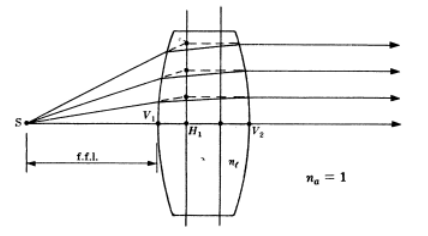
\includegraphics[width=0.9\linewidth]{fig1}
		\caption{\footnotesize{Rayos emergentes en una lente gruesa.}}
		\label{fig:fig1}
	\end{figure}
	
	
	Evidentemente la distancia desde $S$ al v\'ertice $V_{1}$ corresponde a lo que se ha llamado la distancia focal anterior (d.f.a).\\ An\'alogamente, un haz de rayos paralelos incidente convergir\'a en un punto a una distancia m\'as all\'a de $V_{2}$ igual a la distancia focal posterior (d.f.p), como se muestra en la figura \ref{fig:fig2}.
	\begin{figure}[h!]
		\centering
		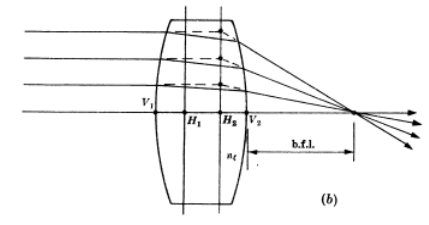
\includegraphics[width=0.9\linewidth]{fig2}
		\caption{\footnotesize{Rayos incidentes en una lente gruesa.}}
		\label{fig:fig2}
	\end{figure}
	Si los rayos entrantes y salientes se prolongan (como se muestra en las lineas punteadas) cada par se cortara sobre una superficie. En la aproximaci\'on paraxial estas superficies se reducen a planos que se conocen como los planos principales primero y segundo; sus puntos de interacci\'on con el eje central $H_{1}$ y $H_{2}$, son los puntos principales primero y segundo, respectivamente. Como m\'etodo practico, para las lentes de vidrio en aire la distancia $\overline{H_{1}H_{2}}$ es aproximadamente igual a una tercera parte del espesor $(d=\overline{V_{1}V_{2}})$ de la lente. Observese que los planos principales no necesariamente están en el interior de la lente. \\
	El caso m\'as simple y m\'as com\'un   es el de la lente de \'indice $n_{\ell}$ sumergida en aire,\\ $n_{a}\approx1$. \\
	La ecuaci\'on de las lentes de Gauss
	\begin{equation}\label{ec1}
		\dfrac{1}{f}=\dfrac{1}{s_{o}}+\dfrac{1}{s_{i}}
	\end{equation}
	se aplica nuevamente siempre a las distancias a objeto e imagen se midan a partir de $H_{1}$ y $H_{2}$ respectivamente. La distancia focal que tambi\'en se mide desde los planos principales esta dada por
	\begin{equation}\label{ec2}
		\dfrac{1}{f}=(n_{\ell}-1)\left[\dfrac{1}{R_{1}}-\dfrac{1}{R_{2}}+\dfrac{(n_{\ell}-1)d}{n_{\ell}R_{1}R_{2}}	\right]
	\end{equation}
	la cual, desde luego, se reduce a la expresi\'on de las lentes delgadas cuando el espesor se hace despreciable $(d\rightarrow 0)$. Los planos principales, a su vez pueden localizarse con respecto a los v\'ertices usando las ecuaciones
	\begin{equation}\label{ec3}
		\overline{V_{1}H_{1}}\equiv h_{1}=-\dfrac{f(n_{\ell}-1)d}{R_{2}n_{\ell}}
	\end{equation}
	\begin{equation}\label{ec4}
	\overline{V_{2}H_{2}}\equiv h_{2}=-\dfrac{f(n_{\ell}-1)d}{R_{1}n_{\ell}}
	\end{equation}
	Tanto $h_{1}$ y $h_{2}$ ser\'an positivos cuando los planos principales est\'an a la derecha de sus respectivos v\'ertices, $V_{1}$ y $V_{2}$. Las relaciones entre las varias distancias se ilustran en la figura \ref{fig:fig3}. Observese que un rayo proveniente de cualquier punto en el plano principal dejar\'a la lente como si fuera originado en un punto situado a la misma altura sobre o debajo del eje, en el segundo plano principal.
	\begin{figure}[h!]
		\centering
		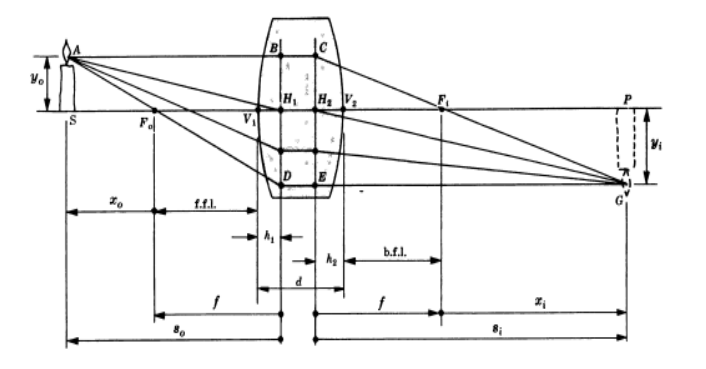
\includegraphics[width=0.9\linewidth]{fig3}
		\caption{\footnotesize{Relaciones entre las varias distancias en una lente gruesa.}}
		\label{fig:fig3}
	\end{figure}
	\subsection{Demostraci\'on de la ecuaci\'on de Newton en lentes gruesas }
	{
		Utilizando las distancias tal y como se definen en la figura \ref{fig:fig3}, se tiene 
		\begin{equation}\label{ec5}
			s_{o}=x_{o}+f
		\end{equation}
		y 
		\begin{equation}\label{ec6}
			s_{i}=x_{i}+f
		\end{equation}
		En consecuencia la ecuaci\'on de Gauss se puede replantear en la forma que sigue
		\begin{equation}\label{ec7}
			f=\dfrac{s_{o}s_{i}}{s_{o}+s_{i}}
		\end{equation}
		sustituyendo las ecuaciones \ref{ec5} y \ref{ec6} en la ecuaci\'on \ref{ec7} se tiene que 
		\begin{equation}
			f=\dfrac{(x_{o}+f)(x_{i}+f)}{(x_{i}+f)+(x_{o}+f)}
		\end{equation}
		0 bien
		\begin{equation}
			f=\dfrac{x_{o}x_{i}+x_{o}f+x_{i}f+f^{2}}{x_{i}+x_{o}+2f}
		\end{equation}
		de donde se sigue que 
		\begin{equation}
		x_{i}f+x_{o}f+2f^{2}=x_{o}x_{i}+x_{o}f+x_{i}f+f^{2}
		\end{equation}
		cancelando t\'erminos iguales se obtiene finalmente que 
		\begin{equation}\label{ec11}
			f^{2}=x_{o}x_{i}
		\end{equation}
		la ecuaci\'on \ref{ec11} es la ecuaci\'on de los lentes en forma newtoniana, se ha probado que en lentes gruesas esta ecuaci\'on sigue siendo igualmente valida.
		
	}
	
}
\section{Experimentos}
{
	Se realizaron dos experimentos los cuales fueron el \emph{m\'etodo del doble desplazamiento} y el m\'etodo \emph{método del deslizador nodal}.
	\subsection{M\'etodo del doble desplazamiento}
	{
		Parte de este experimento utiliza el método de autocolimación, por lo que como se indica en la
		figura \ref{fig:fig4}.
		\begin{itemize}
			\item [ i) ] Primero se localiza, con la ayuda de un espejo, el punto focal primario $F$, al quedar
			definida al lado de la rendija una imagen nítida de la misma. Con la ayuda del riel óptico y su
			escala se anotaron  las posiciones de la rendija, el espejo y el $SOC$, tomando en cuenta en este último
			sus dimensiones y bordes.
			\begin{figure}[h!]
				\centering
				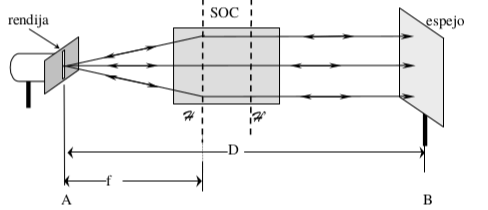
\includegraphics[width=1.0\linewidth]{fig4}
				\caption{\footnotesize{M\'etodo del doble desplazamiento (con espejo).}}
				\label{fig:fig4}
			\end{figure}
			
			\item [ ii) ] Luego se sustituye el  espejo por una pantalla y desplaza hacia la derecha el $SOC$ hasta que se form\'o
			en pantalla una imagen nítida de la rendija. A la distancia así desplazada la denotamos como $x_{o}$. (ver figura \ref{fig:fig5})\\
			\item [ i) ] Luego se puso la lampara y la rendija en la posici\'on $B$ y el espejo en la posici\'on $A$, se repiti\'o el punto i) 
			\item [ iv) ] Sustituimos la  pantalla en punto A y repetimos  ii ) para obtener $x_{i}$.
			\begin{figure}[h!]
				\centering
				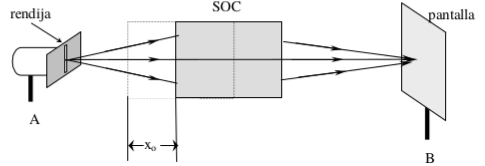
\includegraphics[width=1.0\linewidth]{fig5}
				\caption{\footnotesize{M\'etodo del doble desplazamiento (con pantalla).}}
				\label{fig:fig5}
			\end{figure}
		\end{itemize}
	Los datos obtenidos en este experimento se registraron en la tabla \ref{tabla1}.
	}

	\subsection{Método del deslizador nodal}
	{	
			Se monto el experimento como se indica en la figura \ref{fig:fig6}, y con la ayuda de un láser y
			una pantalla se localizo el mejor punto de enfoque del $SOC$ sobre la pantalla. Aplicamos giros
			pequeños al $SOC$ (indicado como la flecha curva en la figura). Si la imagen sobre la pantalla se
			mueve lateralmente, entonces se desplaza el SOC sobre su montura y repetimos los giros hasta que la
			imagen sobre la pantalla ya no se mov\'ia, entonces el centro de giro es uno de los puntos
			principales, en este caso $H$. Invertimos la cara de incidencia del $SOC$ al láser para repetir
			procedimiento y encontrar $H’$.
			\begin{figure}[h!]
				\centering
				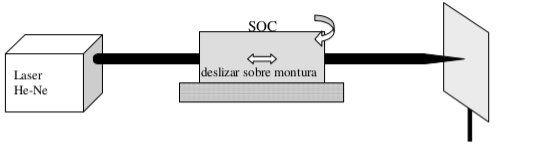
\includegraphics[width=1.0\linewidth]{fig6}
				\caption{\footnotesize{M\'etodo del deslizador nodal.}}
				\label{fig:fig6}
			\end{figure}
		Los datos obtenidos se registraron en a tabla \ref{tabla2}
	}
}


\section{Datos obtenidos}
{
	
		 

Para el m\'etodo del doble desplazamiento se obtuvieron los siguientes datos
\begin{table}[htb]
	\centering
	\begin{tabular}{ccccc}
		N & $f'$ ($cm$) & $s_{o}'$ ($cm$) & $s_{i}'$  ($cm$) & $f''$ ($cm$)  \\ \midrule
		1 &	28.5 & 61.6	& 61.7	& 32.5	\\
		2 &	29.2 & 54.3	& 48.9	& 32.9	\\
		3 &	28.5 & 57.0	& 76.6	& 32.5	\\
		4 &	28.7 & 61.6	& 67.2	& 32.1	\\\hline
	\end{tabular}
	\caption{Datos obtenidos en el m\'etodo del doble desplazamiento} \label{tabla1}
\end{table}

En la tabla anterior se tiene que 

\begin{subequations}
	\begin{equation}\label{ec12a}
		f'=f+d_{1}
	\end{equation}
	
	\begin{equation}\label{ec12b}
		s_{o}'=s_{o}+d_{1}
	\end{equation}
	
	\begin{equation}\label{ec12c}
		s_{i}'=s_{i}+d_{2}
	\end{equation}
	
	\begin{equation}\label{ec12d}
		f''=f+d_{2}
	\end{equation}
\end{subequations}
Note que de las ecuaciones \ref{ec5} y \ref{ec6} se obtienen

\begin{subequations}
	\begin{equation}\label{ec13a}
		x_{o}=s_{o}-f
	\end{equation}
	
	\begin{equation}\label{ec13b}
	x_{i}=s_{i}-f
	\end{equation}
\end{subequations}  

 de \ref{ec12a} y de \ref{ec12b} tenemos que 
\begin{equation}\label{ec14}
	s_{o}'-f'=x_{o}
\end{equation}
adem\'as de \ref{ec12c} y de \ref{ec12d} tenemos que 
\begin{equation}\label{ec15}
s_{i}'-f''=x_{i}
\end{equation}

De estas ecuaciones se obtiene la siguiente tabla 
\begin{table}[htb]
	\centering
	\begin{tabular}{ccccc}
		N & $x_{o}$ ($cm$) & $x_{i}$ ($cm$) & $f^{2}$  ($cm^{2}$) & $f$ ($cm$)  \\ \midrule
		1 &	33.1 & 29.2	& 966.52  & 31.08	\\
		2 &	25.1 & 16.0	& 401.6	  & 20.03	\\
		3 &	28.5 & 44.1	& 1256.85 & 35.45	\\
		4 &	32.9 & 35.1	& 1154.79 & 33.98	\\\hline
	\end{tabular}
	\caption{Datos obtenidos en el m\'etodo del doble desplazamiento despu\'es de usar las ecuaciones \ref{ec12a} a \ref{ec12d}.} \label{tabla2}
\end{table}
\begin{table}[htb]
	\centering
	\begin{tabular}{ccccc}
		N & $s_{o}$ ($cm$) & $s_{i}$ ($cm$) & $x_{o}$  ($cm$) & $x_{i}$ ($cm$)  \\ \midrule
		1  &  &  & & \\
		2  &  &  & & \\
		3  &  &  & & \\
		4  &  &  & & \\\hline
	\end{tabular}
	\caption{Datos obtenidos en el experimento del m\'etodo del deslizador nodal} \label{tabla3}
\end{table}
 
}

\section{Resultados obtenidos}
	{
		De la tabla \ref{tabla2} se obtuvo que $\overline{f}=30.14 cm$
	}

\section{Conclusiones}
	{
		En esta pr\'actica observamos  que por cualquiera de los dos m\'etodos que utilizamos la distancia focal es la misma por lo que podemos decir que los m\'etodos son confiables adem\'as el resultado de las lentes focales obtenidas en los experimentos \'unicamente var\'ian por
	}
	
	\nocite{Hecht}\nocite{Rossi}\nocite{Sears}\nocite{Born}\nocite{Tipler}\nocite{Feynman}\nocite{Res}
	\bibliography{miBiblio.bib}
	\bibliographystyle{plain}


\end{document}